\documentclass{beamer}

\usepackage[left=25mm, top=20mm, right=25mm, bottom=30mm,nohead,nofoot]{geometry}
\usepackage[T2A]{fontenc}
\usepackage[utf8]{inputenc}
\usepackage[english,russian]{babel}
\usepackage[compatibility=false]{caption}
\usepackage{subcaption}
\setcounter{tocdepth}{4}
\usepackage{hyperref}
\hypersetup{unicode=true}
\usepackage{amssymb,latexsym} 
\usepackage{MnSymbol}
\usepackage[nottoc,numbib]{tocbibind}
\usepackage{float}
\usepackage{listings}
\usepackage{multirow}
\usepackage{graphicx}
\usepackage{hhline}
\usepackage{delarray}
\usepackage{color,colortbl}
\usepackage{float}
\usepackage{mathrsfs}
\usepackage[normalem]{ulem}


\usepackage[nottoc]{tocbibind}

\title{Контекстно-свободные грамматики: Выводимость (1.3.1) и Эквивалентные грамматики(1.3.2)}
\author{Попов Иван(4 группа), Реутов Александр, Четвергов Матвей}
\date{17.10.2022}


\begin{document}


	\frame{\titlepage}
	\begin{frame}
    \frametitle{Выводимость в контекстно-свободных грамматиках}
        \textcolor{red}{Дерево разбора}, или \textcolor{red}{дерево вывода} в КГС $G=\langle N,T,R,S \rangle$ - это ориентированное упорядоченное дерево, все узлы которого помечены символами из $N \cup T \cup \{\varepsilon\}$ таким образом, что если в дереве какой-то узел помечен символом $A$, а потомки этого узла помечены символами, образующими слово $\alpha$, то в множестве правил грамматики $R$ существует правило $A \rightarrow \alpha$.
	\end{frame}
	
		\begin{frame}
    \frametitle{Выводимость в контекстно-свободных грамматиках}
        \textcolor{red}{Кроной} дерева вывода назовём цепочку, которая получится, если выписать слева направо метки листьев.\\
        
         \begin{figure}[!tbp]
          \centering
          \begin{minipage}[b]{1\textwidth}
            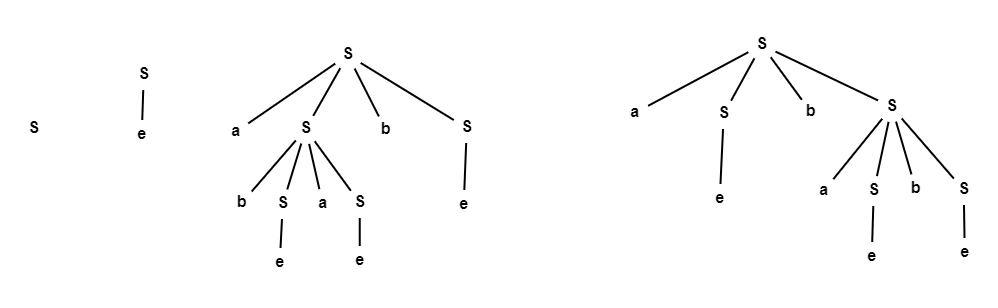
\includegraphics[width=\textwidth]{crown_ex.png}
          \end{minipage}
          \caption{Для грамматики $G$ с правилами $S \longrightarrow aSbS|bSaS|e$}
          \end{figure}
          Для первого дерева крона - S\\
          Для второго - e\\
          Для третьего - abab\\
          Для четвертого - abab
          
	\end{frame}
	
	\begin{frame}{Выводимость в контекстно-свободных грамматиках}
	\textcolor{orange}{Замечание} Третье и четвертое дерево вывода не изоморфны как упорядоченные, но изоморфны как неупорядоченные деревья. 
	
	    
	\end{frame}
	
	\begin{frame}
    \frametitle{Выводимость в контекстно-свободных грамматиках}
        В корневом ориентированном упорядоченном дереве \textcolor{red}{сечением} называется множество узлов, которое содержит ровно по одному узлу из каждого пути корня в лист. В частности, сам корень, а также крона, являются сечениями. \\
        \vspace{3mm}
        Определим \textcolor{red}{сечения} дерева $D$ как цепочку, которая получается конкатенацией (в порядке слева направо) меток вершин, образующих некоторое сечение.\\
        
         \begin{figure}[!tbp]
          \centering
          \begin{minipage}[b]{0.35\textwidth}
            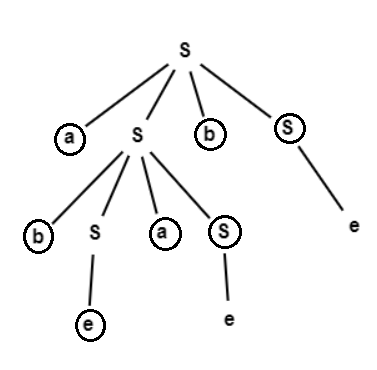
\includegraphics[width=\textwidth]{crown_pruning_ex.png}
          \end{minipage}
          \caption{Пример сечения дерева (множество вершин, обведённых кружками)}
          \end{figure}
          $abaSbS$ - крона сечения дерева вывода.
          
	\end{frame}
	
		\begin{frame}
    \frametitle{Выводимость в контекстно-свободных грамматиках}
        \textcolor{orange}{Теорема.} Если $G=\langle N,T,R,S \rangle$ контекстно-свободная грамматика, то $S \Rightarrow ^\ast \alpha$ тогда и только тогда, когда существует дерево вывода с корнем $S$ и кроной $\alpha \in T^\ast$.\\
        \vspace{3mm}
        \textcolor{orange}{Доказательство.}\\ 1) Пусть $S = \sigma_0, \sigma_1, ... , \sigma_n$ - вывод цепочки  $\alpha$ из $S$ в КС-грамматике $G=\langle N,T,R,S \rangle$. Тогда в $G$ можно построить дерево вывода $D$, для которого $\alpha =\sigma_n$ - крона, а $(\sigma_0, \sigma_1, ... , \sigma_n_-_1)$ - некоторые из крон сечений.\\
        Построим такую последовательность деревьев выводов $D_i (0 \leq i \leq n)$, что $\sigma_i$ - крона дерева $D_i$. Пусть $D_0$ - дерево, состоящее из единственной вершины, помеченной $S$. Пусть $\sigma_i = \beta_i$A$\gamma_i$, применим к $A$ следующее правило: $A \rightarrow X_1, X_2, ..., X_k$. Получается $\sigma_i_+_1 = \beta_iX_1, X_2, ..., X_k\gamma_i$. Тогда дерево $D_i_+_1$ получается из $D_i$ добавлением к листу, помеченному $A$, k прямых потомков, которые помечаются $X_1, X_2, ..., X_k$ соответственно.
        
	\end{frame}
	
	\begin{frame}
    \frametitle{Выводимость в контекстно-свободных грамматиках}
        \textcolor{orange}{Доказательство.}\\ Кроной такого дерева $D_i_+_1$ будет $\sigma_i_+_1$
        2) Пусть теперь $D$ - дерево вывода в КС-грамматике $G=\langle N,T,R,S \rangle$ с кроной $\alpha$. Тогда $S \Rightarrow ^\ast \alpha$.
        Пусть $C_0, C_1, C_2, ..., C_n$ - такая последовательность сечений дерева $D$, что:\\
        \begin{itemize}
        
        \item $C_0$ содержит только корень дерева $D$\\
        \item $C_i_+_1$ для $0 \leq i < n$ получается из $C_i$ заменой одной нетерминальной вершины ее прямыми потомками\\
        \item $C_n$ - крона дерева $D$\\
        \end{itemize}
        Хотя бы одна такая последовательность существует. Если $\sigma_i$ - крона сечения $C_i$, то $\sigma_0, \sigma_1, ..., \sigma_n$ - вывод цепочки $\alpha$ из $S$ в $G$.
        
	\end{frame}
	
		\begin{frame}
    \frametitle{Выводимость в контекстно-свободных грамматиках}
       
         \textcolor{orange}{Замечание.} Теорема утверждает существование дерева вывода, но не утверждает, что такое дерево единственно.
          
	\end{frame}
	
	\begin{frame}
    \frametitle{Выводимость в контекстно-свободных грамматиках}
    \textcolor{orange}{Примечание}\\
    Если во второй части доказательства сечение $C_i_+_1$ получается из $C_i$ заменой самой левой нетерминальной вершины в $C_i$ ее прямыми потомками, то соответствующий вывод $\sigma_0, \sigma_1, ..., \sigma_n$ называется левым (понятие правого вывода вводится аналогично).
    Если $\sigma_0, \sigma_1, ..., \sigma_n$ - левый вывод цепочки $\alpha$, то каждая цепочка $\sigma_i   (0 \leq i < n)$ имеет вид $\beta_iA_i\gamma_i$, где $\beta_i \in T^\ast, A_i \in N$ и $\gamma_i \in (N\cup T)^\ast$
	\end{frame}
	
	\begin{frame}
    \frametitle{Выводимость в контекстно-свободных грамматиках}
    \textcolor{orange}{Пример}\\
    Рассмотрим КС-грамматику $G$ со следующими правилами\\
    \begin{itemize}
        \item $E \rightarrow E + T \ | T$\\
        \item $T \rightarrow T * F \ | F$\\
        \item $F \rightarrow (E) \ | a$\\
    \end{itemize}
    
    \begin{columns}
    \column{.5\textwidth}
    \\Левый вывод\\
      $E \Rightarrow E + T \Rightarrow T + T\\ \Rightarrow F + T \Rightarrow a + T \Rightarrow a + F \Rightarrow a + a$
     \\Правый вывод\\
    $E \Rightarrow E + T \Rightarrow E + F\\ \Rightarrow E + a \Rightarrow T + a \Rightarrow F + a \Rightarrow a + a$ 
    
    \column{.5\textwidth}
    \begin{figure}[!tbp]
          \raggedleft
          \begin{minipage}[b]{0.7\textwidth}
          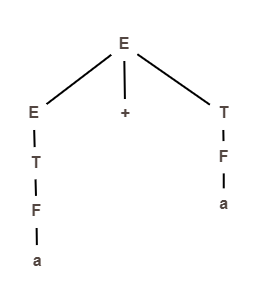
\includegraphics[width=\textwidth]{theorem_ex.png}
          \end{minipage}
          \caption{Пример дерева}
          \end{figure}
    \end{columns}
    
	\end{frame}

		\begin{frame}
    \frametitle{Выводимость в контекстно-свободных грамматиках}
    \textcolor{orange}{Отступление. Аналогия с секвенциями}\\
    \textcolor{red}{Секвенцией} называется выражение вида\\
    Г \vdash  $\Delta$, где Г и $\Delta$ - конечные наборы формул, возможно пустые.
    Г называют антецедентом, а $\Delta$ - сукцедентом.\\
    Примеры секвенций:\\
    $p \land q, \bar p \vdash p \lor \bar q, q$\\
    $p \rightarrow q, \bar p \vdash$\\
    $\vdash \bar p \land \bar q, p \rightarrow q$\\
    В исчислении секвенций имеется 8 правил вывода.\\
    Аксиома исчисления секвенций выглядит следующим образом $A \vdash A$.
    \\или $A$, Г $\vdash A, \Delta$, если рассматривать Г и $\Delta$ как множества, а не последовательности.\\
    Дерево с конечным числом узлов, каждый из которых является секвенцией, называется \textcolor{red}{деревом поиска вывода} секвенции. Если все листья такого дерева являются аксиомами, то такое дерево называют \textcolor{red}{деревом вывода}.
    
	\end{frame}
	
	\begin{frame}
    \frametitle{Выводимость в контекстно-свободных грамматиках}
         \textcolor{orange}{Пример.}\\
         Построим дерево вывода для формулы\\
         $\vdash ((p \rightarrow q) \rightarrow p) \rightarrow p$
          \\\bigskipСтроим дерево поиска вывода
          \\\noindent\rule{4cm}{0.4pt}
          \\\hspace{3mm}$\textcolor{blue}{\vdash} ((p \rightarrow q) \rightarrow p) \textcolor{red}{\rightarrow p}$
          \\\bigskipПрименим правило и получим\\
          \noindent\rule{3cm}{0.4pt}\\
          \hspace{3mm} (p \rightarrow q) \textcolor{red}{\rightarrow p}  \textcolor{blue}{\vdash} p\\
          \noindent\rule{4cm}{0.4pt}
          \\\hspace{3mm}$\vdash ((p \rightarrow q) \rightarrow p) \rightarrow p$
	\end{frame}
	
	\begin{frame}
    \frametitle{Выводимость в контекстно-свободных грамматиках}
           
    \begin{columns}
    \column{.5\textwidth}
       \\\noindent\rule{1.5cm}{0.4pt}\\
         $\textcolor{blue}{\vdash} p \textcolor{red}{\rightarrow} q, p$
         \hspace{0.7cm} $p \vdash p$
         \\\noindent\rule{3cm}{0.4pt}\\
          \hspace{3mm} (p \rightarrow q) \textcolor{red}{\rightarrow p}  \textcolor{blue}{\vdash} p\\
          \noindent\rule{4cm}{0.4pt}
          \\\hspace{3mm}$\vdash ((p \rightarrow q) \rightarrow p) \rightarrow p$
          
          \bigskip
          \\\textcolor{red}{p} $\textcolor{blue}{\vdash}$ q, \textcolor{red}{p}\\
          \\\noindent\rule{1.5cm}{0.4pt}\\
         $\textcolor{blue}{\vdash} p
         \textcolor{red}{\rightarrow} q, p$
         \hspace{0.7cm} $p \vdash p$
         \\\noindent\rule{3cm}{0.4pt}\\
          \hspace{3mm} (p \rightarrow q) \textcolor{red}{\rightarrow p}  \textcolor{blue}{\vdash} p\\
          \noindent\rule{4cm}{0.4pt}
          \\\hspace{3mm}$\vdash ((p \rightarrow q) \rightarrow p) \rightarrow p$
    \column{.5\textwidth}
        \begin{figure}[!tbp]
          \raggedleft
          \begin{minipage}[b]{\textwidth}
          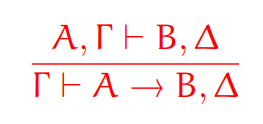
\includegraphics[width=\textwidth]{rule1.png}
          \end{minipage}\\
          \begin{minipage}[b]{\textwidth}
          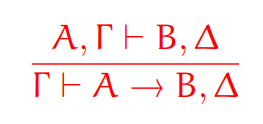
\includegraphics[width=\textwidth]{rule1.png}
          \end{minipage}\\
          \begin{minipage}[b]{\textwidth}
          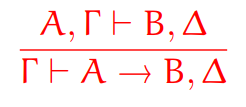
\includegraphics[width=\textwidth]{rule3.png}
          \end{minipage}
          \caption{Используемые правила}
        \end{figure}
    
    \end{columns}
    
         
         
      
	\end{frame}
	
	\begin{frame}
    \frametitle{Выводимость в контекстно-свободных грамматиках}
        \textcolor{orange}{Отступление. Аналогия с орграфами}\\  
        \vspace{3mm}
         \textcolor{orange}{Определение.} Последовательность вершин $(\alpha_0, \alpha_1,...,\alpha_n), n \geq 1$, называется путём (или маршрутом) длины $n$ из вершины $\alpha_0$ в вершину $\alpha_n$, если для каждого $1 \leq i \leq n$, существует дуга, выходящая из вершины $\alpha_i_-_1$ и входящая в вершину $\alpha_i$. Если существует путь из вершины $\alpha_0$ в вершину $\alpha_n$, то говорят, что $\alpha_n$ \textcolor{red}{достижима} из $\alpha_0$.\\
         \vspace{3mm}
         Таким образом, понятие достижимости соответствует выводимости в грамматиках
 
	\end{frame}
	
	\begin{frame}{Пример для аналогии с орграфами}
	   \textcolor{orange}{Пример}: Пусть $G_1=\langle\{E\}, \{a,+,*,(,)\}, \{E \to E + E \  |\ E * E\ |\ ( E ) \ |\  a\}, E\rangle$
          \begin{figure}[!tbp]
          \centering
            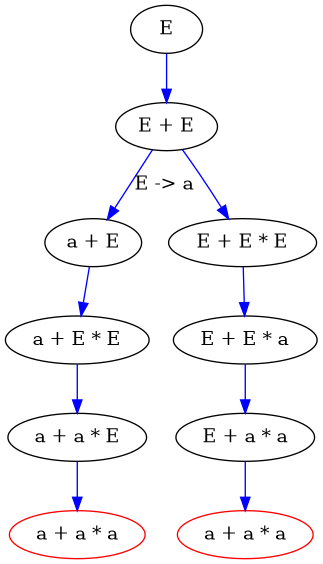
\includegraphics[width=0.35\textwidth]{orgraph_ex.png}
          \caption{Орграф, соответствующий одному из левых и правых выводов для $a+a*a$ в $G_1$}
        \end{figure}
	\end{frame}
	
	
	\begin{frame}
    \frametitle{Эквивалентные грамматики}
        Далее пойдет рассказ об эквивалентных, но отличающихся грамматиках на примере арифметических выражений.
	\end{frame}
	
	\begin{frame}
    \frametitle{Эквивалентные грамматики}
         Если $\mathfrak{L}(G_1)=\mathfrak{L}(G_2)$, то грамматики $G_1$ и $G_2$ называются \textcolor{red}{эквивалентными}, т.е. порождающими один и тот же язык.\\
         \vspace{3mm}
         \textcolor{orange}{Пример}: $G_1=\langle\{E\}, \{a,+,*,(,)\}, R_1, E\rangle$, где $R_1$ это: 
         $$
         E \to E + E \  |\ E * E\ |\ ( E ) \ |\  a
         $$
         и $G_2=\langle\{E,T\}, \{a,+,*,(,)\}, R_2, E\rangle$, где $R_2$ это
        \begin{gather}
         E \to E + T \  |\ E * T\ |\ T \nonumber \\
         T \to (E) \ |\  a  \nonumber
        \end{gather}
         
	\end{frame}
	
	\begin{frame}
    \frametitle{Неоднозначность $G_1$}
        В то же время, $G_1$ является \textcolor{red}{неоднозначной}, т.е. для некоторых слов существуют более одного вывода. Так, для выражения $a + a * a$ есть два дерева вывода:
        
        \begin{figure}[!tbp]
          \centering
          \begin{minipage}[b]{0.4\textwidth}
            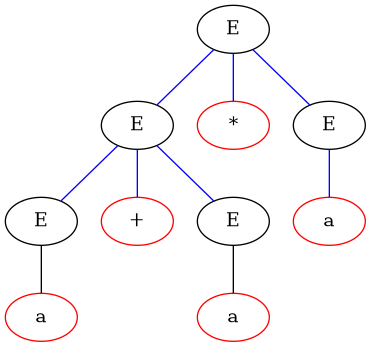
\includegraphics[width=\textwidth]{g1_ex1.png}
          \end{minipage}
          \hfill
          \begin{minipage}[b]{0.4\textwidth}
            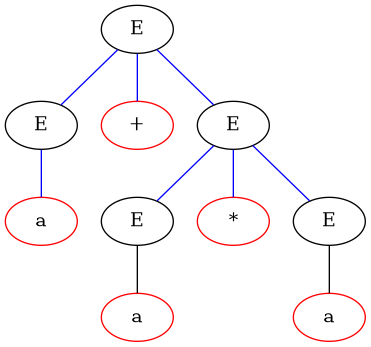
\includegraphics[width=\textwidth]{g1_ex2.png}
          \end{minipage}
          \caption{Деревья вывода для $a+a*a$ в $G_1$}
        \end{figure}
	\end{frame}
	
	\begin{frame}{Грамматики арифметических выражений}
	    Проблемы с неоднозначными грамматиками начинаются, когда доходит дело до практических аспектов и синтаксического анализа.\\
	    \vspace{3mm}
	    К тому же, для определенного подкласса однозначных грамматик существуют эффективные алгоритмы парсинга\\
	    \vspace{3mm}
	    Так, при разборе синтаксическим анализатором левого дерева с прошлого слайда получится выражение, эквивалентное $(a+a)*a$, в то время как выражение для правого дерева будет $a+(a*a)$.\\
	     
	\end{frame}

    	
	\begin{frame}{Грамматики арифметических выражений}
	    Грамматика $G_2$ однозначна, т.к. симметричные правила вывода $E \to E + E$ и $E \to E * E$ из $G_1$ заменены на несимметричные $E \to E + T$ и $E \to E * T$. 
	     \begin{figure}[!tbp]
          \centering
            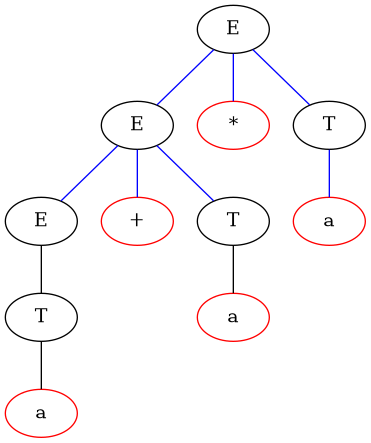
\includegraphics[width=0.4\textwidth]{g2_ex.png}
          \caption{Дерево вывода для $a+a*a$ в $G_2$}
        \end{figure}
        Стоит заметить, что из-за введения еще одной переменной размер дерева вывода увеличился
	\end{frame}

	\begin{frame}{Грамматики арифметических выражений}
    Тем не менее, обе грамматики $G_1$ и $G_2$ все равно обладают одним недостатком - у операций $+$ и $*$ одинаковый приоритет.\\
    \vspace{3mm}
    \textcolor{orange}{Отступление} Если внимательнее посмотреть на $G_2$, можно заметить, что там приоритет операций задается порядком, в котором они идут в записи выражения.\\
    \vspace{3mm}
    Так, выражение $a+a*a$ эквивалентно при разборе $(a+a)*a$, но если поменять порядок на $a*a+a$, то получится $(a*a)+a$
	\end{frame}
	
	\begin{frame}{Грамматики арифметических выражений}
	Чтобы получить однозначную грамматику с правильным приоритетом операций, нужно добавить еще одну переменную.\\
	\vspace{3mm}
	Пусть грамматика $G_3=\langle\{E,T,F\}, \{a,+,*,(,)\}, R_3, E\rangle$, где $R_3$ это 
	    \begin{gather}
         E \to E + T \ |\ T \nonumber \\
         T \to T * F \ |\  F  \nonumber \\
         F \to (E) \ |\  a  \nonumber
        \end{gather}
	
	\end{frame}
    \begin{frame}{Грамматики арифметических выражений}
    В грамматике $G_3$ умножение приоритетнее сложения, и при разборе выражения $a+a*a$ результат будет согласовываться с правилами арифметики.
       \begin{figure}[!tbp]
          \centering
            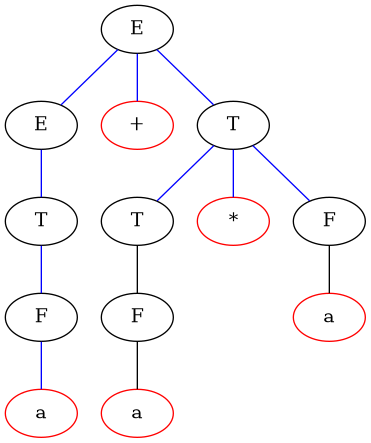
\includegraphics[width=0.4\textwidth]{g3_ex.png}
          \caption{Дерево вывода для $a+a*a$ в $G_3$}
        \end{figure}
   Так, один язык генерируют 3 грамматики, отличающиеся размером дерева, количеством переменных и правил вывода. 
   \end{frame}
    

\end{document}